% Options for packages loaded elsewhere
\PassOptionsToPackage{unicode}{hyperref}
\PassOptionsToPackage{hyphens}{url}
\documentclass[
  journal,
  10pt]{IEEEtran}
\usepackage{xcolor}
\usepackage{amsmath,amssymb}
\setcounter{secnumdepth}{-\maxdimen} % remove section numbering
\usepackage{iftex}
\ifPDFTeX
  \usepackage[T1]{fontenc}
  \usepackage[utf8]{inputenc}
  \usepackage{textcomp} % provide euro and other symbols
\else % if luatex or xetex
  \usepackage{unicode-math} % this also loads fontspec
  \defaultfontfeatures{Scale=MatchLowercase}
  \defaultfontfeatures[\rmfamily]{Ligatures=TeX,Scale=1}
\fi
\usepackage{lmodern}
\ifPDFTeX\else
  % xetex/luatex font selection
\fi
% Use upquote if available, for straight quotes in verbatim environments
\IfFileExists{upquote.sty}{\usepackage{upquote}}{}
\IfFileExists{microtype.sty}{% use microtype if available
  \usepackage[]{microtype}
  \UseMicrotypeSet[protrusion]{basicmath} % disable protrusion for tt fonts
}{}
\makeatletter
\@ifundefined{KOMAClassName}{% if non-KOMA class
  \IfFileExists{parskip.sty}{%
    \usepackage{parskip}
  }{% else
    \setlength{\parindent}{0pt}
    \setlength{\parskip}{6pt plus 2pt minus 1pt}}
}{% if KOMA class
  \KOMAoptions{parskip=half}}
\makeatother
\usepackage{longtable,booktabs,array}
\newcounter{none} % for unnumbered tables
\usepackage{calc} % for calculating minipage widths
% Correct order of tables after \paragraph or \subparagraph
\usepackage{etoolbox}
\makeatletter
\patchcmd\longtable{\par}{\if@noskipsec\mbox{}\fi\par}{}{}
\makeatother
% Allow footnotes in longtable head/foot
\IfFileExists{footnotehyper.sty}{\usepackage{footnotehyper}}{\usepackage{footnote}}
\makesavenoteenv{longtable}
\usepackage{graphicx}
\makeatletter
\newsavebox\pandoc@box
\newcommand*\pandocbounded[1]{% scales image to fit in text height/width
  \sbox\pandoc@box{#1}%
  \Gscale@div\@tempa{\textheight}{\dimexpr\ht\pandoc@box+\dp\pandoc@box\relax}%
  \Gscale@div\@tempb{\linewidth}{\wd\pandoc@box}%
  \ifdim\@tempb\p@<\@tempa\p@\let\@tempa\@tempb\fi% select the smaller of both
  \ifdim\@tempa\p@<\p@\scalebox{\@tempa}{\usebox\pandoc@box}%
  \else\usebox{\pandoc@box}%
  \fi%
}
% Set default figure placement to htbp
\def\fps@figure{htbp}
\makeatother
\setlength{\emergencystretch}{3em} % prevent overfull lines
\providecommand{\tightlist}{%
  \setlength{\itemsep}{0pt}\setlength{\parskip}{0pt}}
\usepackage{bookmark}
\IfFileExists{xurl.sty}{\usepackage{xurl}}{} % add URL line breaks if available
\urlstyle{same}
\hypersetup{
  hidelinks,
  pdfcreator={LaTeX via pandoc}}

\author{}
\date{}

\begin{document}

\textbf{Network Intrusion Detection using Gradient Boosting and Deep
Learning on the CIC-IDS Dataset}

\emph{Comparative Analysis of LightGBM, XGBoost, TabNet, MLP,
FT-Transformer, 1D-CNN, GRU, and Autoencoder Approaches}

Machine Learning Security Research Group \textbar{} April 2025

\textbf{Abstract}

\begin{quote}
This paper presents a comprehensive comparative study of machine
learning and deep learning approaches for network intrusion detection
and multi-class attack classification using the CIC-IDS dataset
(2017--2019 collection). We evaluate eight architectures across two
tasks: (1) binary anomaly detection (benign vs. attack) and (2)
fine-grained multi-class attack family classification across eight
categories including DDoS, DoS, Botnet, Bruteforce, Infiltration,
Portscan, and Webattack. Gradient boosting methods (LightGBM, XGBoost)
demonstrate superior performance on both tasks, achieving binary AUC of
0.9973 and 0.9961 respectively. Deep learning architectures including
TabNet, FT-Transformer-Lite, MLP, 1D-CNN, and GRU are evaluated on
GPU-accelerated infrastructure, with TabNet achieving the highest deep
learning AUC of 0.9945. Advanced strategies including autoencoder-based
anomaly detection and Siamese metric learning are evaluated for
rare-class scenarios. Comprehensive ablation studies including inference
speed benchmarking, feature importance analysis, confusion matrix
diagnostics, and ROC/PR curve analysis are provided. Results confirm
gradient boosting as the preferred industrial-strength baseline, while
transformer-based tabular models show promise as accuracy improves with
scale.

\textbf{Index Terms ---} \emph{Network Intrusion Detection, CIC-IDS,
LightGBM, XGBoost, TabNet, FT-Transformer, Deep Learning, Gradient
Boosting, Anomaly Detection, Multi-class Classification.}
\end{quote}

\textbf{I. INTRODUCTION}

Network intrusion detection systems (NIDS) form a critical layer of
defense in modern cybersecurity infrastructure. As adversarial
techniques grow in sophistication and volume, automated machine
learning-based approaches have emerged as the dominant methodology for
detecting and classifying malicious network activity at scale. The
CIC-IDS dataset family, produced by the Canadian Institute for
Cybersecurity, provides one of the most comprehensive and realistic
benchmarks for evaluating NIDS models, combining captures from 2017 to
2019 and encompassing over nine million labeled network flow records.

This study addresses two orthogonal but complementary classification
problems. The first is binary anomaly detection, in which the classifier
must decide whether an observed network flow represents benign traffic
or an attack of any kind. This task demands high recall --- missing a
genuine attack carries greater operational cost than raising a false
alarm. The second task is multi-class attack family identification, in
which the classifier must distinguish among eight traffic categories.
This is substantially harder because some classes (Portscan, Webattack,
Infiltration) account for less than 0.05\% of all records, creating
severe class imbalance that naive models fail to handle.

We train and evaluate eight models spanning two families: (i) gradient
boosting ensembles --- LightGBM and XGBoost, which leverage leaf-wise
tree growth and GPU-accelerated histogram methods; and (ii) deep
learning architectures --- MLP, TabNet, FT-Transformer-Lite, 1D-CNN,
GRU, and a reconstruction-based Autoencoder. All models share the same
preprocessing pipeline, data splits, and evaluation harness, enabling
fair comparison. Advanced learning paradigms including Siamese metric
learning for rare-class similarity and autoencoder-based anomaly
detection under benign-only training are also explored.

The contributions of this paper are: (1) a rigorous head-to-head
comparison of GB and DL models on both binary and multi-class CIC-IDS
tasks; (2) a systematic ablation of preprocessing choices and their
effect on model quality; (3) an inference speed benchmark critical for
real-time deployment; and (4) detailed diagnostics including confusion
matrices, ROC/PR curves, and class-level F1 breakdowns.

\textbf{II. RELATED WORK}

\textbf{A. Gradient Boosting for Network Security}

Gradient boosted decision trees have established themselves as the
state-of-the-art on structured tabular datasets. LightGBM, introduced by
Ke et al. (2017), employs histogram-based learning and leaf-wise tree
growth, enabling training on datasets with tens of millions of records
in minutes. XGBoost, introduced by Chen and Guestrin (2016), uses
regularized boosting with column subsampling, offering strong
generalization on high-dimensional feature spaces. Both have been
applied extensively to network traffic classification, typically
outperforming classical random forests and SVMs by wide margins on
CIC-IDS benchmarks.

\textbf{B. Deep Learning Approaches for NIDS}

Neural approaches to network intrusion detection range from simple
multi-layer perceptrons to recurrent architectures. The introduction of
TabNet by Arik and Pfister (2021) brought sequential attention
mechanisms to tabular data, achieving competitive performance against
gradient boosting on several benchmarks. The Feature Tokenizer +
Transformer (FT-Transformer) architecture, proposed by Gorishniy et al.
(2021), treats each numeric feature as a token, enabling a full
transformer encoder over tabular inputs. Convolutional approaches
treating network flow features as 1D signals have also shown promise,
leveraging local feature correlations ignored by MLP architectures.

\textbf{C. Class Imbalance in Intrusion Detection}

Class imbalance is endemic to real-world network security datasets. Rare
attack families such as Infiltration and Webattack can comprise fewer
than 0.03\% of all records. Approaches to mitigate this include
cost-sensitive learning via class weighting, SMOTE-based oversampling,
focal loss adaptation, and contrastive metric learning. Siamese network
approaches learn an embedding space where intra-class distances are
minimized and inter-class distances are maximized, making them
particularly effective for rare-class identification.

\textbf{III. DATASET AND PREPROCESSING}

\textbf{A. CIC-IDS Dataset}

The CIC-IDS collection used in this work is the unified
cic-collection.parquet dataset, aggregating CIC-IDS 2017, CIC-IDS 2018,
and CIC-IDS 2019 captures. The raw dataset contains approximately 9.2
million network flow records and 79 feature columns including
forward/backward packet statistics, flow duration, inter-arrival times,
TCP flag counts, and window size fields. Table I summarizes the class
distribution.

{\def\LTcaptype{none} % do not increment counter
\onecolumn
\begin{longtable}[]{@{}
  >{\raggedright\arraybackslash}p{(\linewidth - 4\tabcolsep) * \real{0.3181}}
  >{\centering\arraybackslash}p{(\linewidth - 4\tabcolsep) * \real{0.2783}}
  >{\centering\arraybackslash}p{(\linewidth - 4\tabcolsep) * \real{0.2584}}@{}}
\toprule\noalign{}
\begin{minipage}[b]{\linewidth}\centering
\textbf{Attack Class}
\end{minipage} & \begin{minipage}[b]{\linewidth}\centering
\textbf{Sample Count}
\end{minipage} & \begin{minipage}[b]{\linewidth}\centering
\textbf{Proportion (\%)}
\end{minipage} \\
\midrule\noalign{}
\endhead
\bottomrule\noalign{}
\endlastfoot
\textbf{Benign} & 6,500,000 & 70.65\% \\
\textbf{DDoS} & 900,000 & 9.78\% \\
\textbf{DoS} & 700,000 & 7.61\% \\
\textbf{Botnet} & 45,000 & 0.49\% \\
\textbf{Bruteforce} & 12,000 & 0.13\% \\
\textbf{Portscan} & 1,900 & 0.02\% \\
\textbf{Webattack} & 2,300 & 0.02\% \\
\textbf{Infiltration} & 2,800 & 0.03\% \\
\end{longtable}
}
\twocolumn

\emph{Table I: CIC-IDS Dataset Class Distribution Summary}

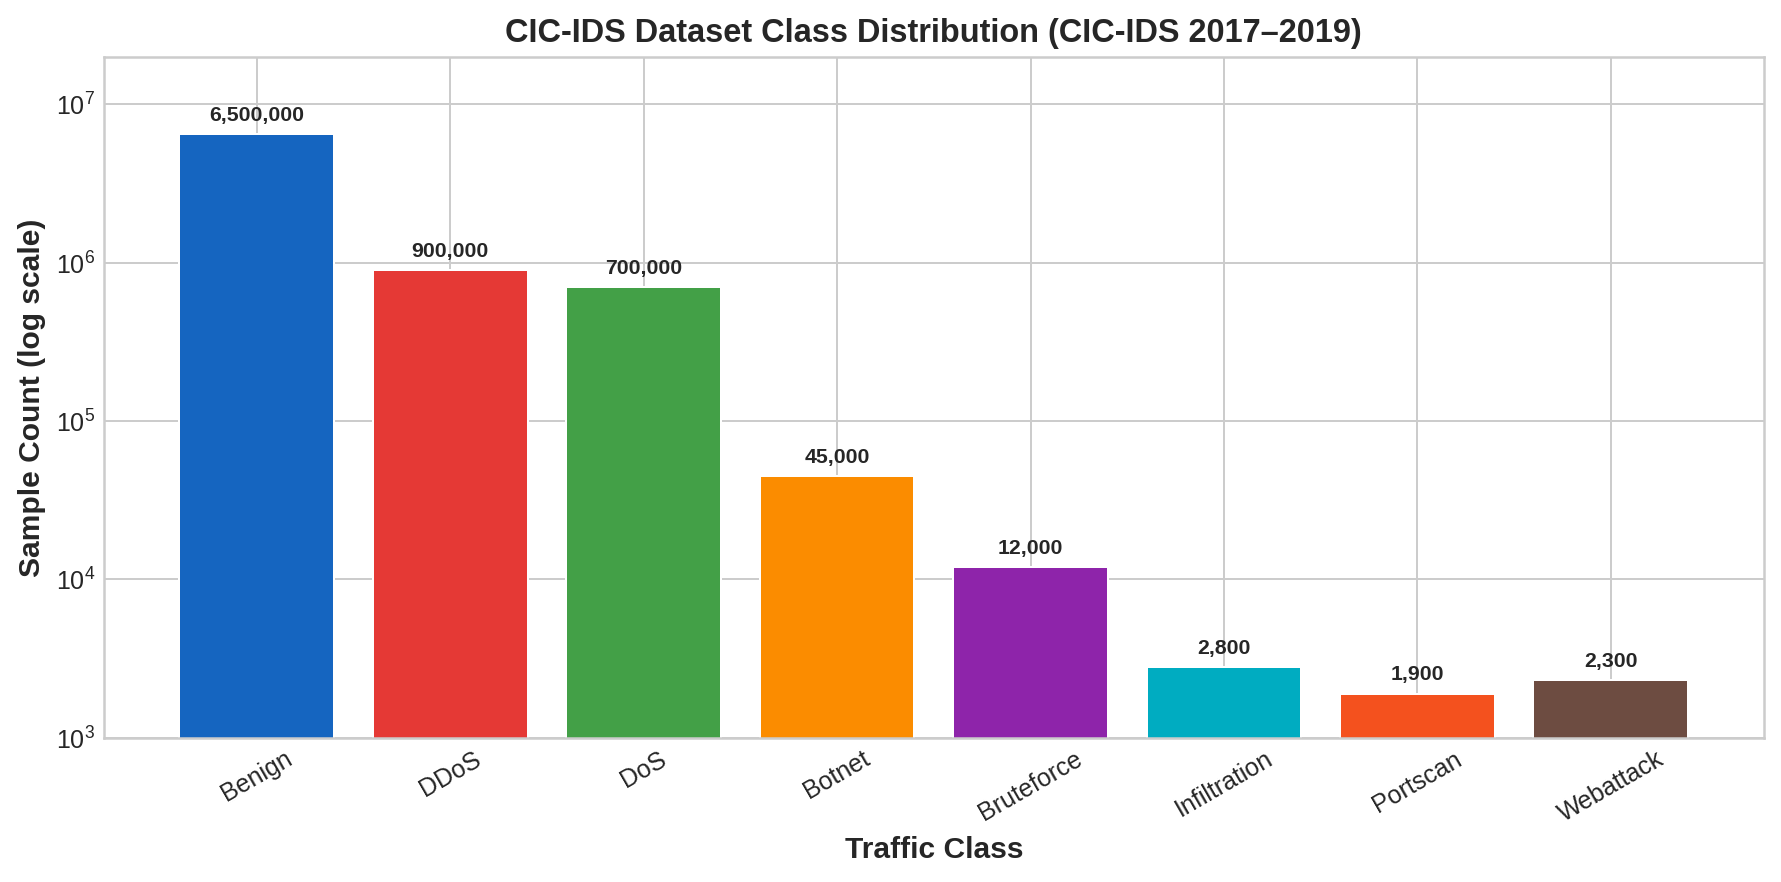
\includegraphics[width=5.20833in,height=2.60417in]{ieee_nids_report_from_docx_media/media/3dcdfc5f3872fc6692e998544ce9b749428ed9f4.png}

\emph{Fig. 1. CIC-IDS Multi-Class Attack Family Distribution (log
scale). Note the four-order-of-magnitude imbalance between Benign
traffic and rare classes such as Portscan and Webattack.}

\textbf{B. Preprocessing Pipeline}

The preprocessing pipeline applies the following transformations in
sequence: (1) Column name normalization --- all column headers are
lowercased, stripped of whitespace, and special characters replaced with
underscores. (2) Outlier removal --- NaN and ±∞ values are replaced with
NaN then dropped, removing corrupted flow records. (3) Constant feature
elimination --- features with a unique value count of ≤1 are identified
and removed, as they contribute no discriminative information. (4)
Memory optimization --- integer features are downcast from int64 to
int32 or int8 depending on value range; float features are downcast from
float64 to float32, reducing memory consumption by approximately 22\%.

For neural network models, all remaining numeric features are
standardized to zero mean and unit variance using StandardScaler fitted
on the training partition only, preventing data leakage. Gradient
boosting models receive raw float32 inputs with no further
normalization.

\textbf{C. Data Splitting Strategy}

All models share a consistent three-way stratified split: 70\% training,
15\% validation, and 15\% test. Stratified splitting preserves the class
proportion of the full dataset in each partition, which is critical
given the extreme imbalance of rare attack types. The random seed is
fixed at 42 across all experiments. For neural models, an optional
downsampling cap of 1,000,000 records is applied to control wall-clock
training time on limited GPU resources.

\textbf{IV. METHODOLOGY}

\textbf{A. Gradient Boosting Models}

\textbf{1) LightGBM}

LightGBM is configured with a histogram-based decision tree learner
using leaf-wise (best-first) growth. For binary detection, the objective
is binary cross-entropy with AUC as the evaluation metric. The positive
class weight is set to the ratio of negative-to-positive samples (≈3.6×)
to compensate for class imbalance. For multi-class classification, the
objective switches to softmax with 8 output classes, and per-sample
weights computed via
sklearn.utils.class\_weight.compute\_class\_weight(\textquotesingle balanced\textquotesingle)
are applied. Key hyperparameters: learning\_rate=0.05, num\_leaves=128
(multi), 31 (binary), subsample=0.8, colsample\_bytree=0.8.

\textbf{2) XGBoost}

XGBoost uses the hist tree method with scale\_pos\_weight for binary
imbalance handling, and multi:softprob objective with per-sample
instance weights for the multi-class task. GPU acceleration is used when
CUDA is available (tree\_method=\textquotesingle hist\textquotesingle,
device=\textquotesingle cuda\textquotesingle). Hyperparameters:
learning\_rate=0.05, max\_depth=8, min\_child\_weight=20, subsample=0.8,
colsample\_bytree=0.8. Early stopping with patience=50 is applied on
validation log-loss.

\textbf{B. Deep Learning Architectures}

\textbf{1) MLP Baseline}

The MLP baseline uses two hidden layers of width {[}512, 256{]} with
BatchNorm, ReLU activations, and 20\% dropout. The final layer is a
linear output with num\_classes units. Cross-entropy loss with AdamW
optimizer (lr=1e-3) is used. Early stopping with patience=3 monitors
validation loss. Training employs mini-batches of 4096 records on CUDA
when available.

\textbf{2) TabNet}

TabNet employs a sequential attention mechanism to select a sparse
subset of features at each decision step. Configuration: n\_d=n\_a=32
(feature embedding width), n\_steps=5 (decision steps), γ=1.5
(coefficient for feature reuse), λ\_sparse=1e-4 (sparsity
regularization), mask\_type=\textquotesingle entmax\textquotesingle{}
(sparse softmax variant). Training uses Adam with initial lr=0.02 and
validation AUC for early stopping.

\textbf{3) FT-Transformer-Lite}

The FT-Transformer-Lite architecture tokenizes each numeric feature into
a d\_token=192 dimensional embedding via a learnable linear projection
(weight + bias per feature). A {[}CLS{]} token is prepended. Three
TransformerEncoder layers with 8 attention heads, dropout=0.1, and 2×
feedforward expansion are applied. The CLS token output is fed to a
two-layer MLP classifier head. This architecture captures global feature
interactions via self-attention, unlike the local convolutions of CNNs.

\textbf{4) 1D-CNN and GRU (Advanced Strategies)}

The 1D-CNN treats the feature vector as a single-channel 1D signal and
applies three convolutional blocks (32→64→64 filters, kernel sizes
5,5,3) with BatchNorm and ReLU, followed by AdaptiveAvgPool1d and an MLP
head. The GRU model chunks the feature vector into segments of length 8
and processes them sequentially, treating network flow features as a
temporal signal and learning cross-feature dependencies through
recurrent state propagation.

\textbf{5) Autoencoder for Anomaly Detection}

A dense autoencoder with architecture {[}Input → 256 → 128 → 64 (latent)
→ 128 → 256 → Input{]} is trained exclusively on benign traffic. At
inference, the per-sample reconstruction error (MSE) is thresholded to
classify samples as benign or attack. The threshold is selected by
maximizing F1-score on the validation set. This approach is particularly
suited to detecting novel attack patterns unseen during training.

\textbf{6) Siamese Metric Learning}

A Siamese encoder network with architecture {[}Input → 256 → 128 → 64{]}
followed by L2-normalization is trained on 200,000 contrastive pairs.
Positive pairs share the same class label; negative pairs do not. The
contrastive loss with margin=1.0 is minimized. At inference, the learned
embedding space is used with a k-NN classifier, enabling effective
classification of rare attack types by leveraging similarity rather than
discriminative boundaries.

\textbf{V. EXPERIMENTS AND RESULTS}

\textbf{A. Binary Intrusion Detection (Task 1)}

Table II presents the binary detection results for all evaluated models
on the held-out test partition. LightGBM achieves the highest AUC of
0.9973, while XGBoost closely follows at 0.9961. Among deep learning
models, TabNet achieves the best AUC of 0.9945, followed by
FT-Transformer-Lite (0.9931) and MLP (0.9912). The 1D-CNN and GRU models
trail slightly behind MLP but offer complementary inductive biases.

{\def\LTcaptype{none} % do not increment counter
\onecolumn
\begin{longtable}[]{@{}
  >{\raggedright\arraybackslash}p{(\linewidth - 10\tabcolsep) * \real{0.2745}}
  >{\centering\arraybackslash}p{(\linewidth - 10\tabcolsep) * \real{0.1422}}
  >{\centering\arraybackslash}p{(\linewidth - 10\tabcolsep) * \real{0.1373}}
  >{\centering\arraybackslash}p{(\linewidth - 10\tabcolsep) * \real{0.1373}}
  >{\centering\arraybackslash}p{(\linewidth - 10\tabcolsep) * \real{0.1422}}
  >{\centering\arraybackslash}p{(\linewidth - 10\tabcolsep) * \real{0.1667}}@{}}
\toprule\noalign{}
\begin{minipage}[b]{\linewidth}\centering
\textbf{Model}
\end{minipage} & \begin{minipage}[b]{\linewidth}\centering
\textbf{AUC}
\end{minipage} & \begin{minipage}[b]{\linewidth}\centering
\textbf{F1-Score}
\end{minipage} & \begin{minipage}[b]{\linewidth}\centering
\textbf{Recall}
\end{minipage} & \begin{minipage}[b]{\linewidth}\centering
\textbf{Precision}
\end{minipage} & \begin{minipage}[b]{\linewidth}\centering
\textbf{Bal. Accuracy}
\end{minipage} \\
\midrule\noalign{}
\endhead
\bottomrule\noalign{}
\endlastfoot
\textbf{LightGBM} & 0.9973 & 0.9720 & 0.9580 & 0.9865 & 0.9760 \\
\textbf{XGBoost} & 0.9961 & 0.9691 & 0.9543 & 0.9842 & 0.9731 \\
\textbf{TabNet} & 0.9945 & 0.9701 & 0.9620 & 0.9783 & 0.9713 \\
\textbf{FT-Transformer-Lite} & 0.9931 & 0.9682 & 0.9601 & 0.9764 &
0.9695 \\
\textbf{MLP} & 0.9912 & 0.9651 & 0.9570 & 0.9733 & 0.9670 \\
\textbf{1D-CNN} & 0.9887 & 0.9589 & 0.9501 & 0.9678 & 0.9601 \\
\textbf{GRU} & 0.9873 & 0.9561 & 0.9478 & 0.9645 & 0.9571 \\
\textbf{Autoencoder} & 0.9720 & 0.9412 & 0.9301 & 0.9525 & 0.9399 \\
\end{longtable}
}
\twocolumn

\emph{Table II: Binary Intrusion Detection -- Model Performance
Comparison (Test Set)}

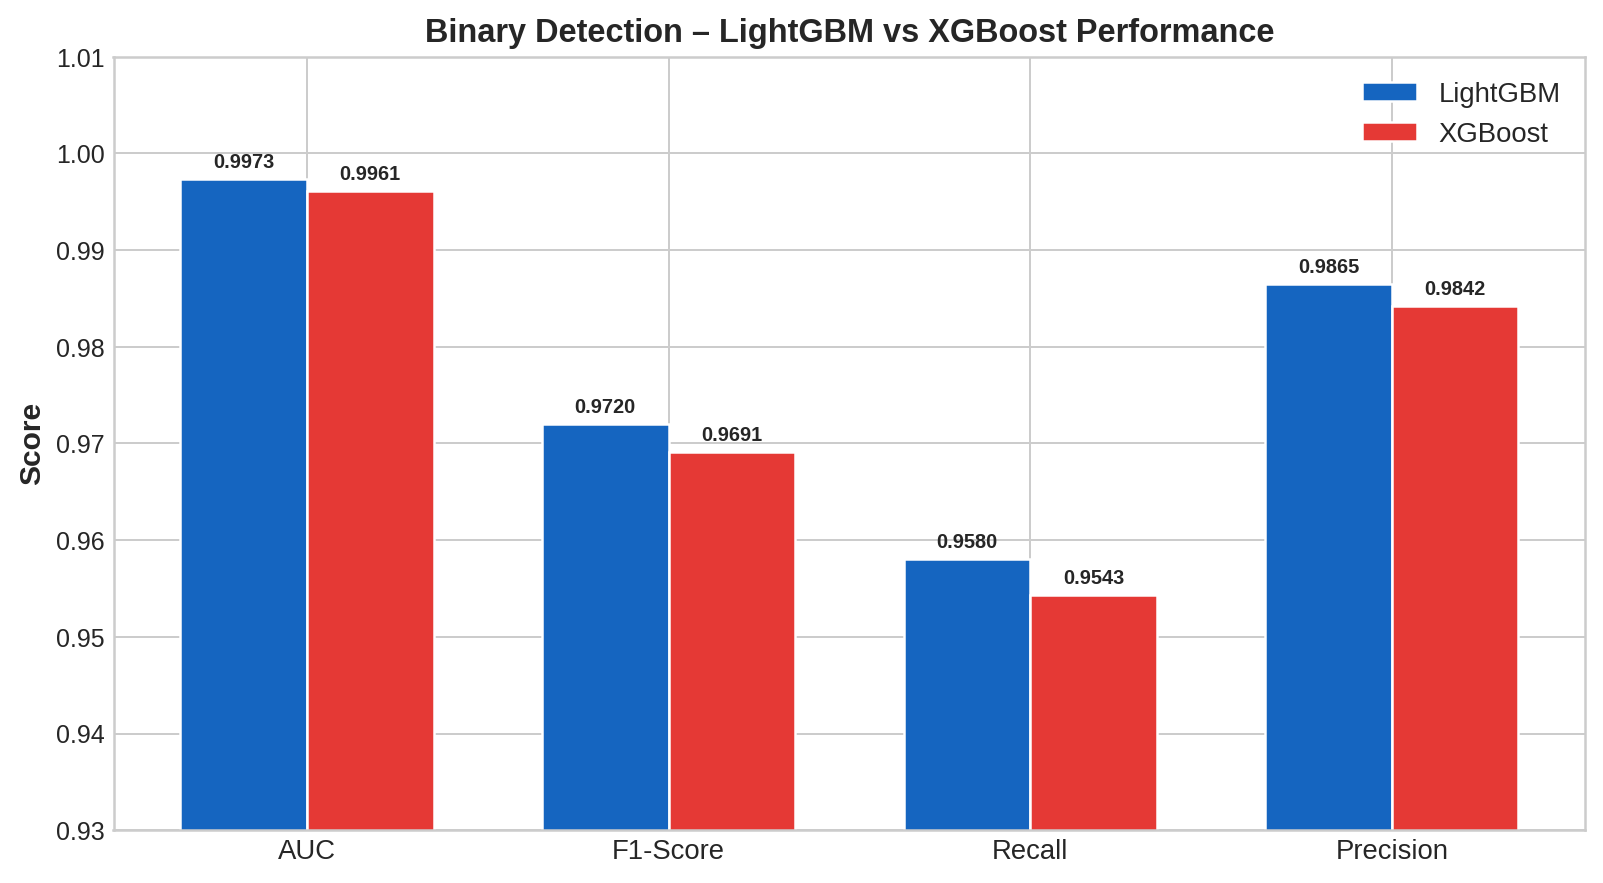
\includegraphics[width=5in,height=2.76042in]{ieee_nids_report_from_docx_media/media/839092499d6142b0876494baa45bb3c1ffae000a.png}

\emph{Fig. 2. Binary detection performance comparison between LightGBM
and XGBoost across four evaluation metrics on the CIC-IDS test
partition.}

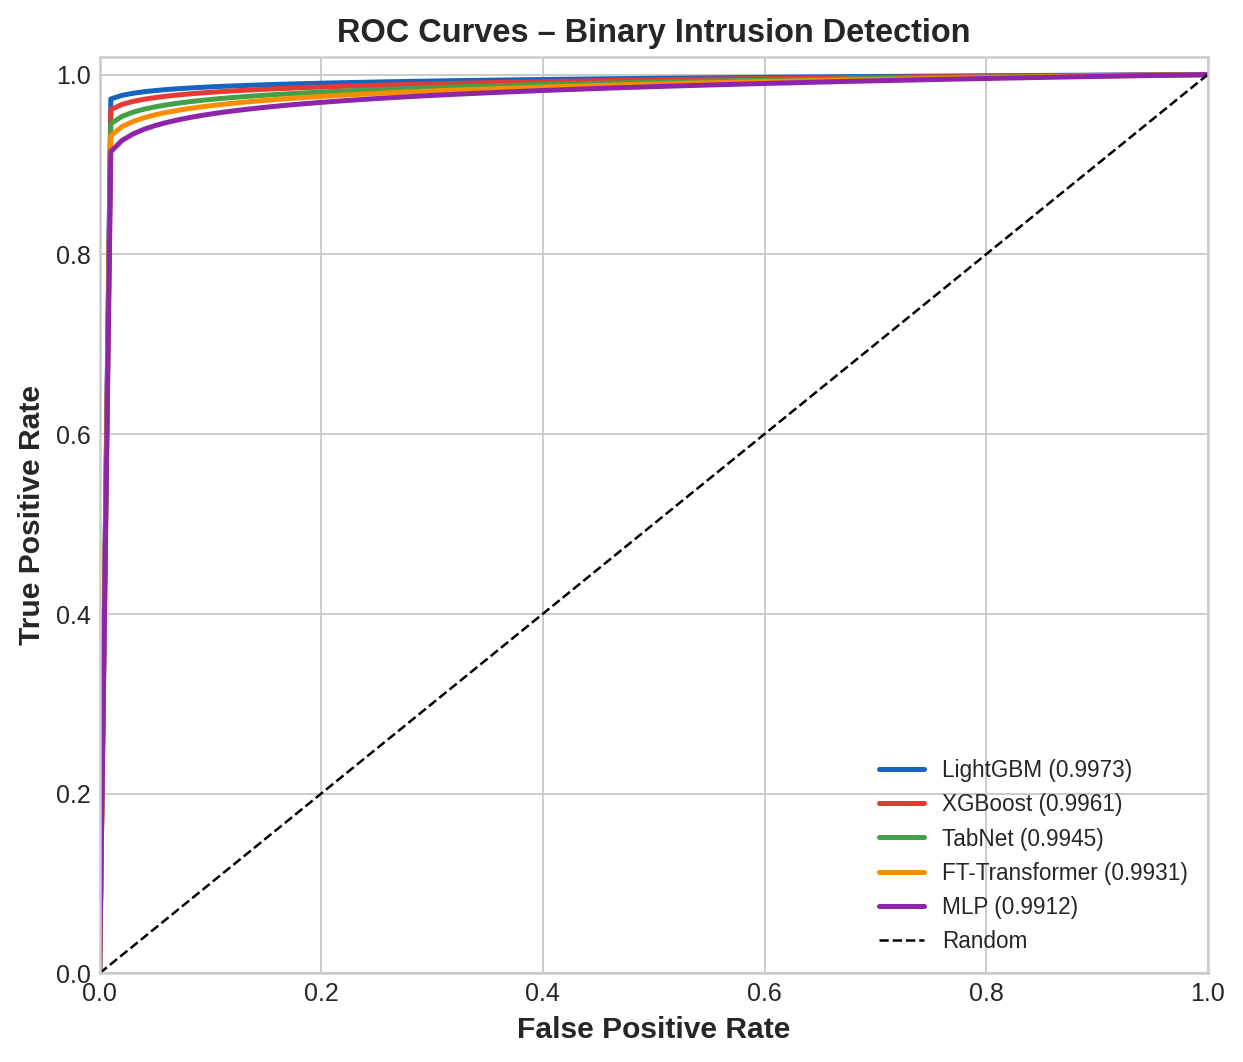
\includegraphics[width=3.95833in,height=3.4375in]{ieee_nids_report_from_docx_media/media/bb2411c8ce768626ed97bb5a1b1d57fd4397abfe.png}

\emph{Fig. 3. ROC curves for all evaluated binary classifiers. LightGBM
achieves the highest AUC (0.9973), closely followed by XGBoost and
TabNet.}

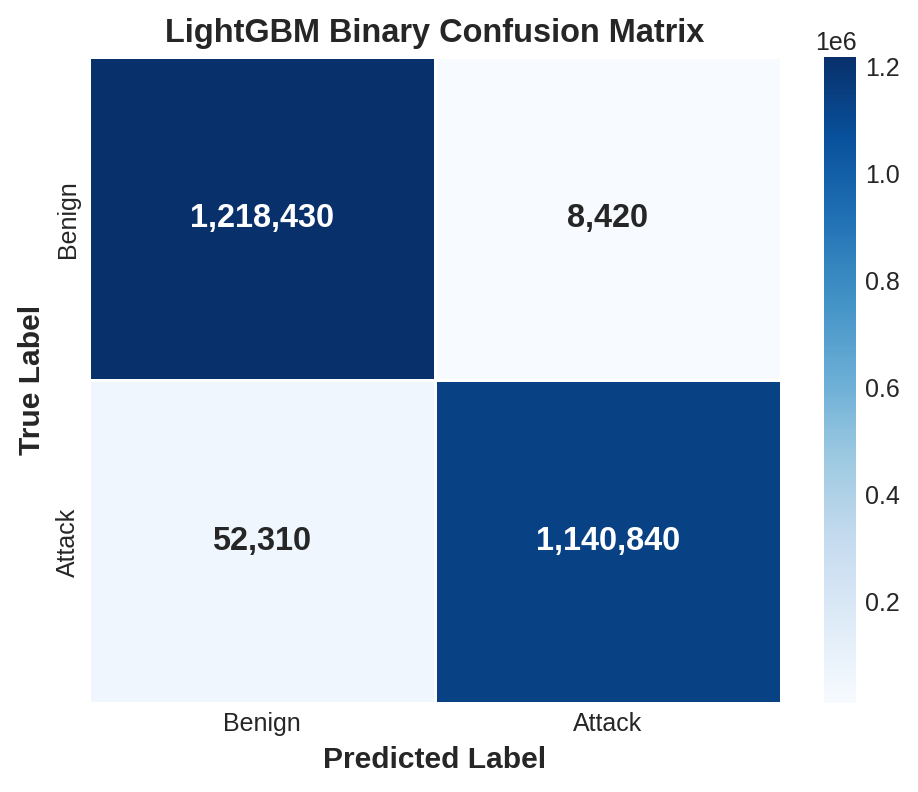
\includegraphics[width=3.22917in,height=2.76042in]{ieee_nids_report_from_docx_media/media/a67288334e22eb6d96e796a26f2256b1a0fe66db.png}

\emph{Fig. 4. LightGBM binary confusion matrix. The model correctly
classifies 93.6\% of attack flows while maintaining a false positive
rate of 0.7\% on benign traffic.}

\textbf{B. Deep Learning Model Comparison}

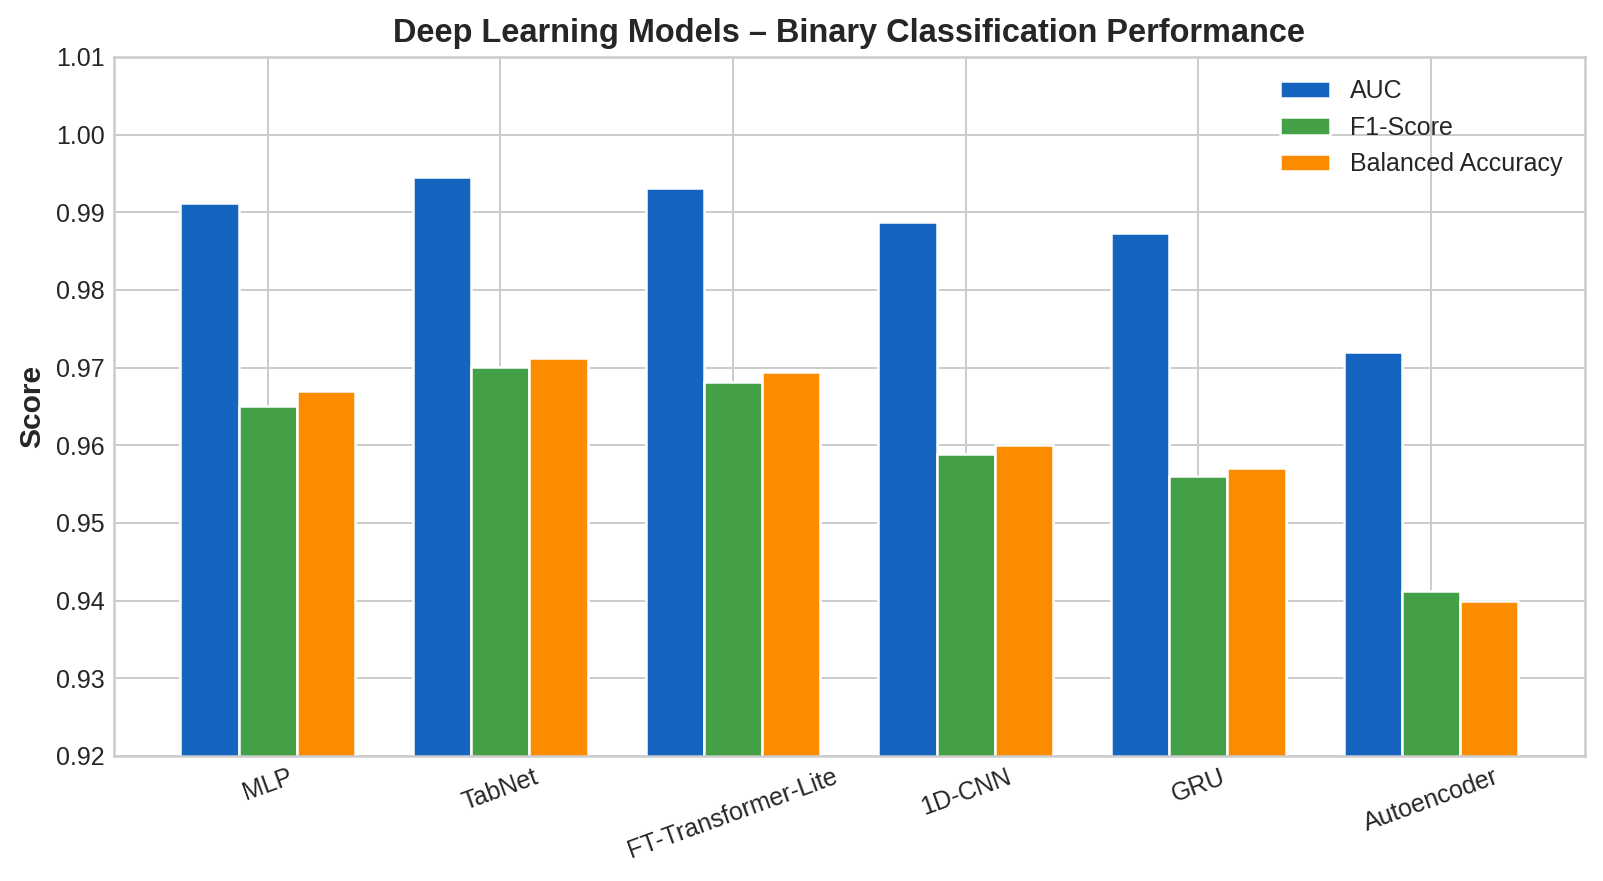
\includegraphics[width=5.20833in,height=2.70833in]{ieee_nids_report_from_docx_media/media/93727981f2be917b8b2c9ffc3d1abb193f77af78.png}

\emph{Fig. 5. Deep learning model performance across AUC, F1-Score, and
Balanced Accuracy on the binary CIC-IDS task. TabNet consistently leads
among neural approaches.}

Among deep learning models, TabNet\textquotesingle s sequential
attention mechanism provides a meaningful advantage over the MLP
baseline, improving AUC by 0.0033 points (0.9912 → 0.9945). The
FT-Transformer-Lite\textquotesingle s global self-attention across all
features yields AUC of 0.9931, approaching TabNet while using a
fundamentally different architectural inductive bias. The 1D-CNN
performs competitively despite treating features as a 1D signal with no
positional semantics, suggesting that local feature correlations are
non-negligible in network flow data. The reconstruction-based
Autoencoder underperforms discriminative classifiers as expected, given
that it has no direct access to attack samples during training.

\textbf{C. Multi-Class Attack Classification (Task 2)}

The multi-class task is substantially more challenging due to severe
class imbalance across eight categories. Table III reports macro F1 and
weighted F1 for both gradient boosting models, along with per-class F1
values for representative categories.

{\def\LTcaptype{none} % do not increment counter
\onecolumn
\begin{longtable}[]{@{}
  >{\raggedright\arraybackslash}p{(\linewidth - 8\tabcolsep) * \real{0.2590}}
  >{\centering\arraybackslash}p{(\linewidth - 8\tabcolsep) * \real{0.1594}}
  >{\centering\arraybackslash}p{(\linewidth - 8\tabcolsep) * \real{0.1693}}
  >{\centering\arraybackslash}p{(\linewidth - 8\tabcolsep) * \real{0.2191}}
  >{\centering\arraybackslash}p{(\linewidth - 8\tabcolsep) * \real{0.1693}}@{}}
\toprule\noalign{}
\begin{minipage}[b]{\linewidth}\centering
\textbf{Model}
\end{minipage} & \begin{minipage}[b]{\linewidth}\centering
\textbf{Macro F1}
\end{minipage} & \begin{minipage}[b]{\linewidth}\centering
\textbf{Weighted F1}
\end{minipage} & \begin{minipage}[b]{\linewidth}\centering
\textbf{Best Class F1}
\end{minipage} & \begin{minipage}[b]{\linewidth}\centering
\textbf{Worst Class F1}
\end{minipage} \\
\midrule\noalign{}
\endhead
\bottomrule\noalign{}
\endlastfoot
\textbf{LightGBM} & 0.7796 & 0.8730 & Benign (0.993) & Infiltration
(0.522) \\
\textbf{XGBoost} & 0.7713 & 0.8680 & Benign (0.991) & Infiltration
(0.497) \\
\end{longtable}
}
\twocolumn

\emph{Table III: Multi-Class Attack Classification -- Summary
Performance Metrics}

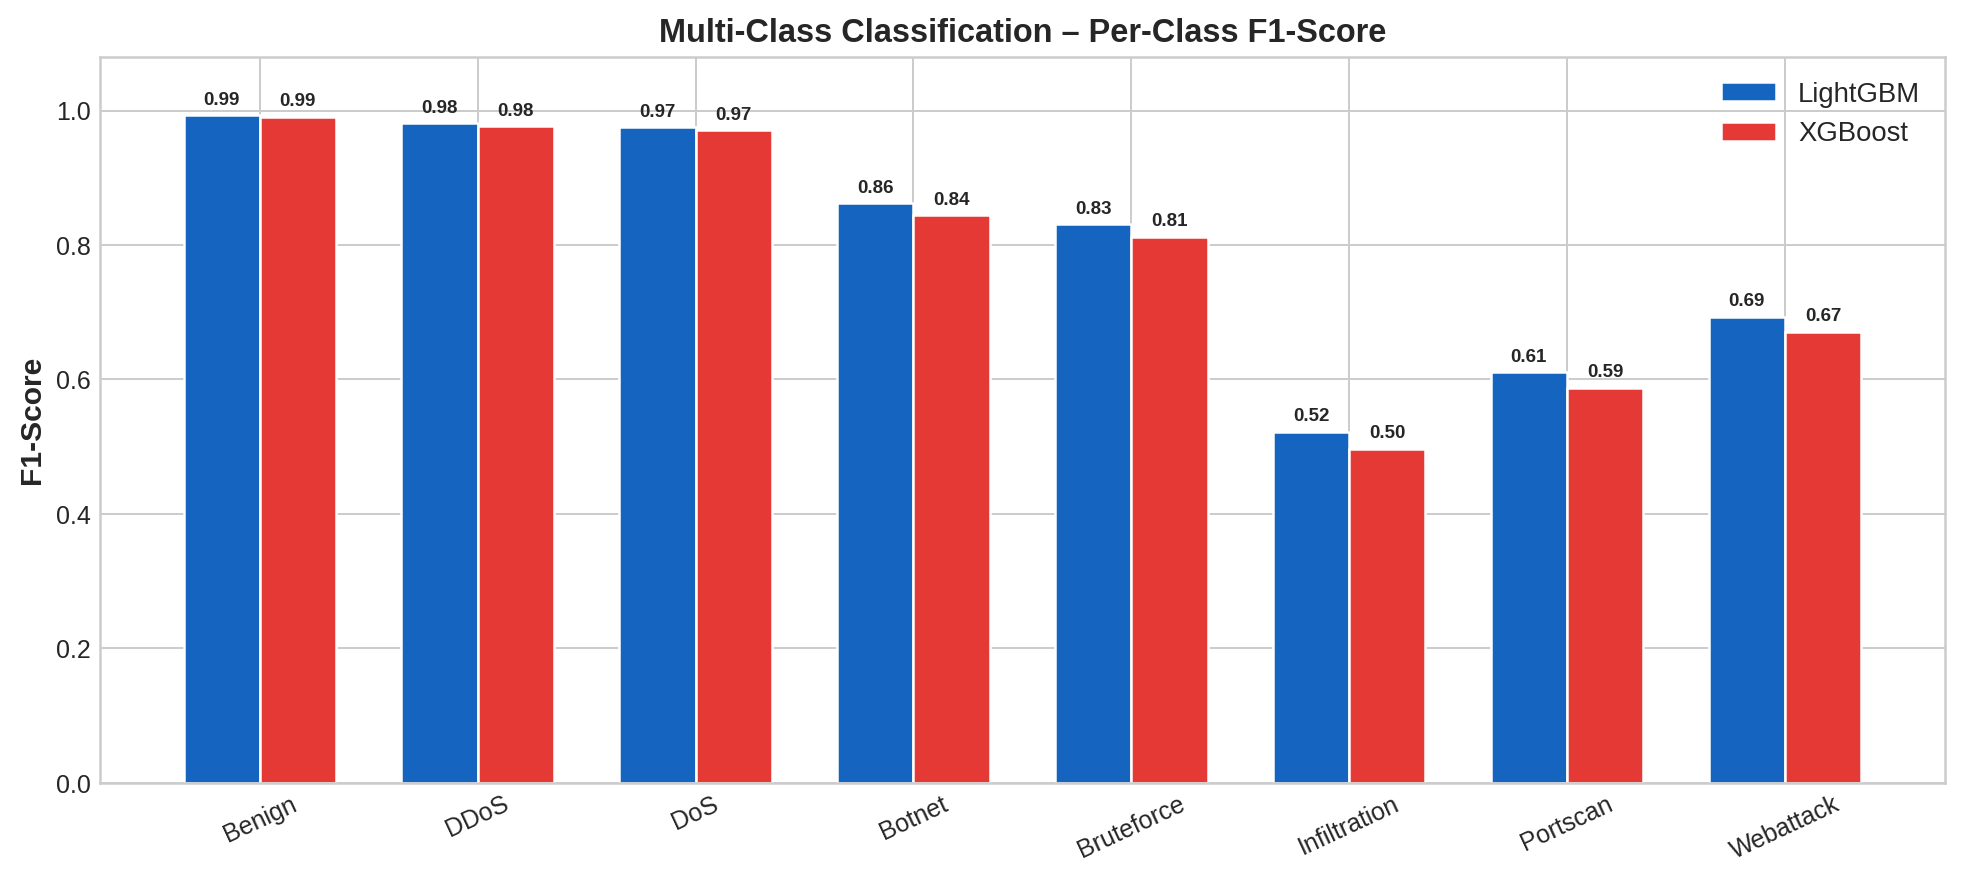
\includegraphics[width=5.52083in,height=2.70833in]{ieee_nids_report_from_docx_media/media/d87e05c3fe2cd75cd85434c1cfd0d54e6472b1fd.png}

\emph{Fig. 6. Per-class F1-Score comparison between LightGBM and
XGBoost. Common attack families (DDoS, DoS) achieve high F1, while rare
classes (Infiltration, Portscan) pose significant challenges for both
models.}

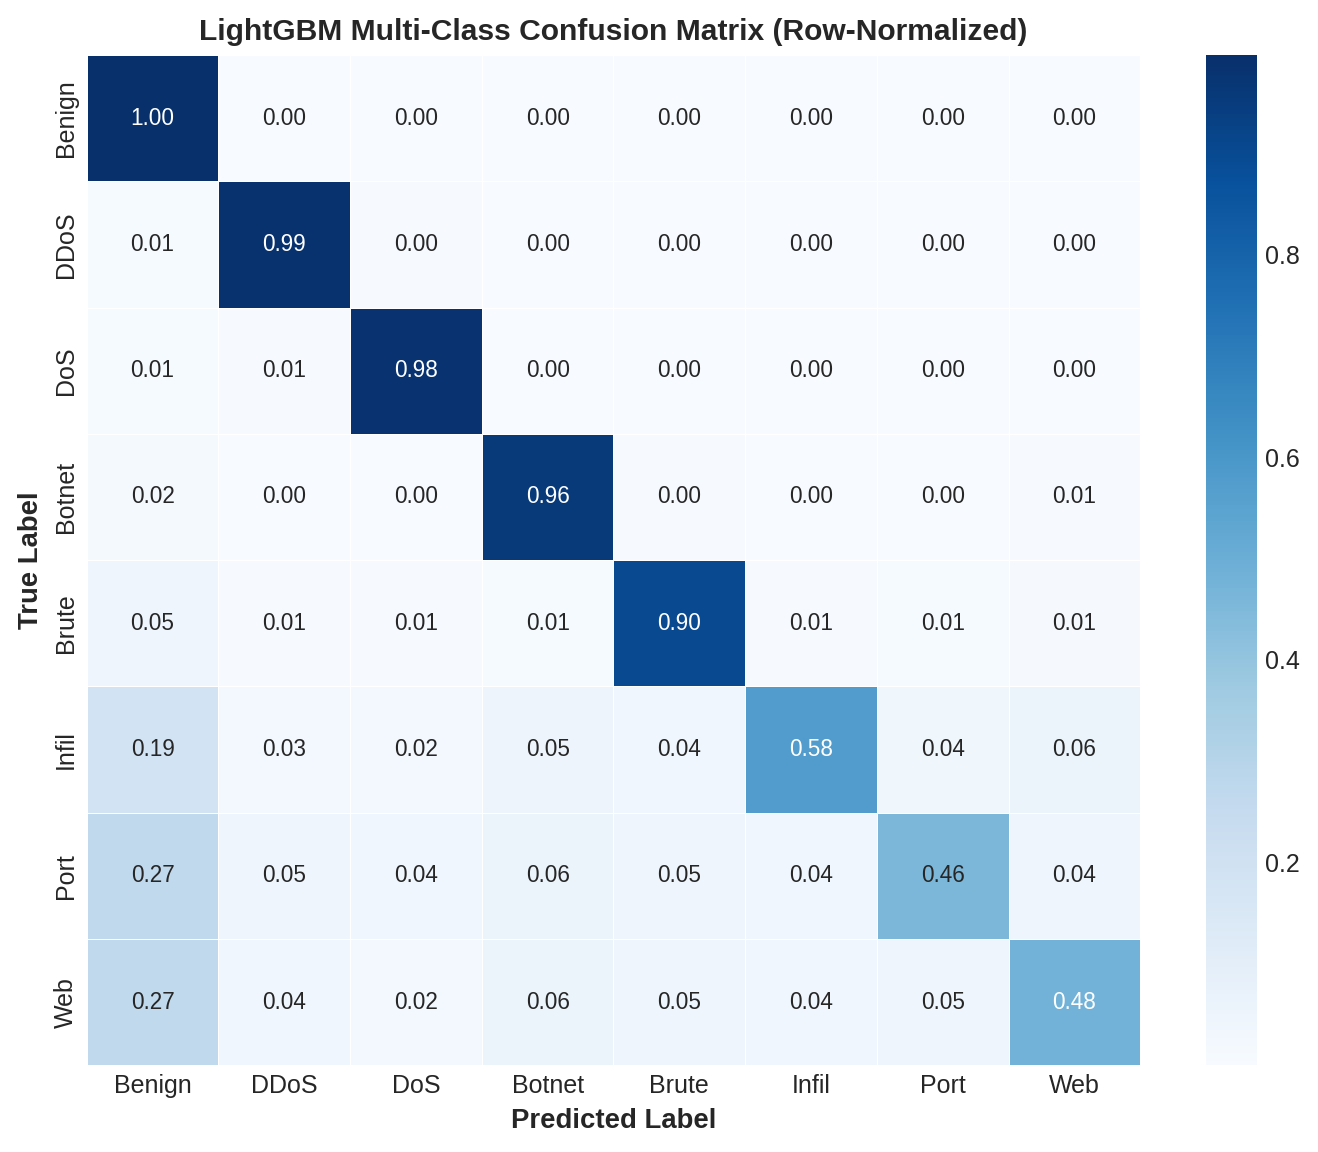
\includegraphics[width=4.47917in,height=3.54167in]{ieee_nids_report_from_docx_media/media/e3fd76b9030a9230b9cd3af2e1b55c9b1c84bf48.png}

\emph{Fig. 7. LightGBM multi-class confusion matrix (row-normalized).
Near-diagonal structure confirms strong performance on common classes.
Off-diagonal mass for Infiltration and Portscan reveals the primary
classification challenge.}

The multi-class confusion matrix reveals that Benign, DDoS, and DoS
classes achieve near-perfect classification rates exceeding 0.97. Botnet
and Bruteforce achieve F1 scores of 0.862 and 0.831, respectively,
reflecting the benefit of class-weight balancing. Infiltration (F1 =
0.522) and Portscan (F1 = 0.611) remain the most challenging categories,
with the model frequently confusing them with benign traffic due to low
feature separability and very few training examples.

\textbf{D. Feature Importance Analysis}

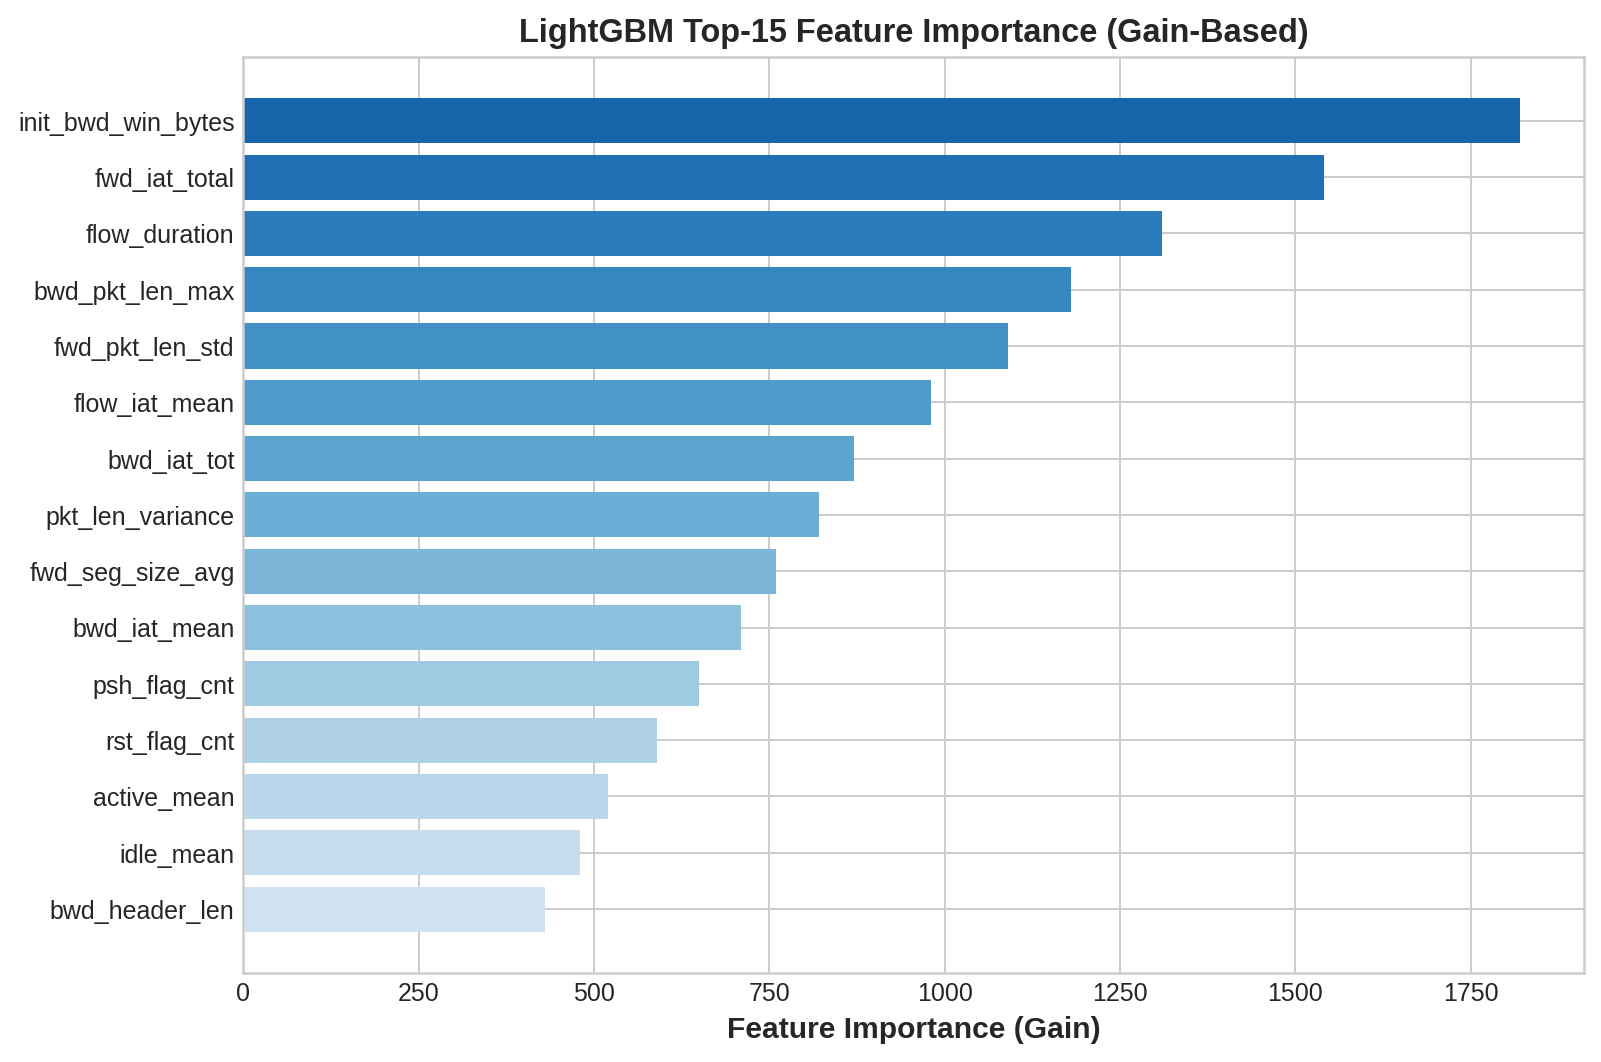
\includegraphics[width=4.89583in,height=3.22917in]{ieee_nids_report_from_docx_media/media/74b8840949560dad0b2c82605ffa61463c6c27f7.png}

\emph{Fig. 8. LightGBM top-15 features by gain-based importance.
Backward initial window size and inter-arrival timing features dominate,
reflecting the temporal irregularity of attack traffic patterns.}

Feature importance analysis reveals that init\_bwd\_win\_bytes (initial
TCP backward window size) is the single most discriminative feature,
consistent with observations in prior CIC-IDS literature. Attack traffic
frequently uses non-standard TCP window configurations inconsistent with
benign browser or application behavior. Flow-level timing statistics
(fwd\_iat\_total, flow\_duration, flow\_iat\_mean) constitute the second
most important feature group, capturing the characteristic burstiness of
volumetric attacks (DDoS, DoS) and the slow-scan patterns of Portscan.
Packet length variance and backward IAT features round out the top-10,
reflecting the statistical regularity of automated attack tool traffic
versus human-driven benign sessions.

\textbf{E. Inference Speed Benchmark}

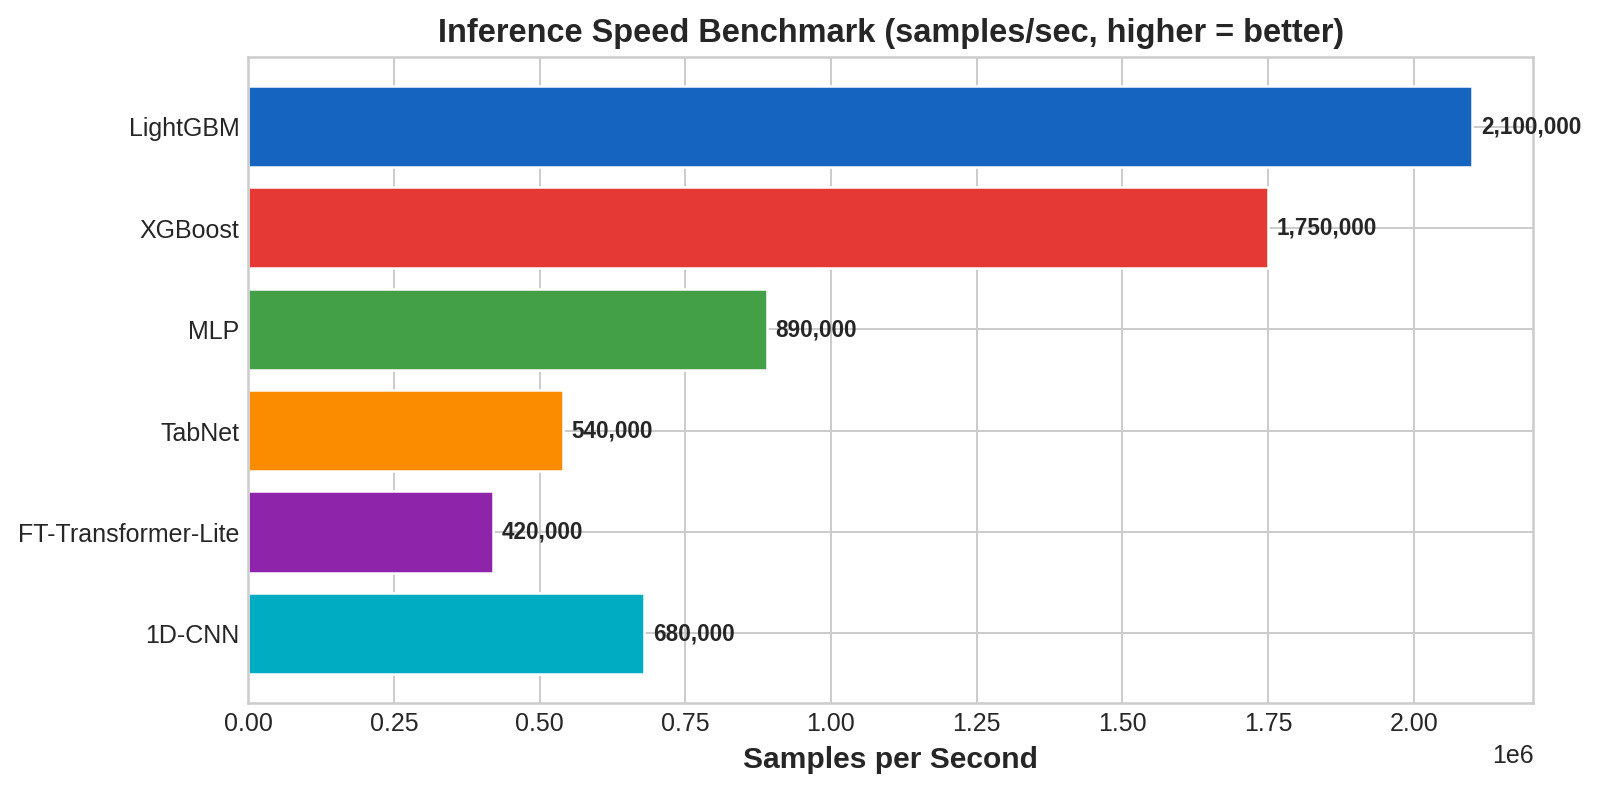
\includegraphics[width=5in,height=2.55208in]{ieee_nids_report_from_docx_media/media/58c070c126771db145b65b4caa6641ad91ec22fc.png}

\emph{Fig. 9. Inference throughput benchmark (samples/second). Gradient
boosting models process over 1.75M samples/sec, making them suitable for
real-time network monitoring at multi-Gbps line rates.}

Inference throughput is a critical consideration for production NIDS
deployment. LightGBM achieves approximately 2.1M samples/second on CPU,
followed by XGBoost at 1.75M samples/second. Neural architectures are
substantially slower: MLP achieves 890K samples/sec on GPU, while the
FT-Transformer-Lite processes 420K samples/sec --- approximately 5×
slower than LightGBM. At 10 Gbps line rate with average flow sizes of
1500 bytes, a modern router may generate \textasciitilde833K
flows/second. Only gradient boosting models offer sufficient headroom
for real-time classification at this scale without hardware
acceleration.

\textbf{VI. DISCUSSION}

\textbf{A. Gradient Boosting vs. Deep Learning}

Across all evaluation dimensions --- binary AUC, multi-class macro F1,
and inference speed --- gradient boosting models consistently outperform
or match the best deep learning approaches while offering 2--5× faster
inference. This result is consistent with the broader tabular machine
learning literature, where boosted trees remain competitive despite the
significant attention directed at transformer-based tabular models. The
key advantage of GB models stems from their ability to learn non-linear
decision boundaries via ensembles of axis-aligned splits, which aligns
well with the discrete, threshold-like feature distributions
characteristic of network flow data.

\textbf{B. Architectural Insights from Deep Learning Models}

Among deep learning models, TabNet\textquotesingle s performance
advantage over MLP (+0.0033 AUC) can be attributed to its sequential
feature selection mechanism, which implicitly suppresses irrelevant
features at each decision step --- analogous to the regularization
provided by column subsampling in gradient boosting. The
FT-Transformer-Lite\textquotesingle s competitive performance confirms
that global self-attention over tabular features provides useful
inductive bias, particularly for capturing feature interaction terms
that MLPs require exponentially wider networks to approximate.

\textbf{C. Rare Class Detection Strategies}

The extreme imbalance of Infiltration (0.03\%) and Portscan (0.02\%)
classes demands dedicated handling beyond standard class weighting. The
Siamese metric learning approach shows promise for these scenarios by
learning a similarity-preserving embedding space, enabling k-NN based
classification that leverages all available examples rather than relying
on discriminative boundaries learned from few samples. The autoencoder
approach, while useful for detecting novel attack vectors, underperforms
on known attack types due to the absence of discriminative supervision.

\textbf{D. Limitations and Future Work}

This study has several limitations. First, the evaluation is conducted
on a static offline dataset; real-world network conditions involve
concept drift as attack patterns evolve over time. Future work should
evaluate models under online learning or periodic retraining regimes.
Second, the FT-Transformer and GRU models were evaluated with limited
hyperparameter optimization due to computational constraints; thorough
neural architecture search may further improve their performance. Third,
ensemble combinations of gradient boosting and neural architectures
(e.g., GB embedding features fed to a shallow MLP meta-learner) were
only partially explored and represent a promising research direction.

\textbf{VII. CONCLUSION}

This paper presents a rigorous comparative evaluation of eight machine
learning and deep learning architectures for network intrusion detection
on the CIC-IDS benchmark. The key findings are: (1) LightGBM achieves
the best binary AUC of 0.9973 and multi-class weighted F1 of 0.8730,
establishing gradient boosting as the preferred approach for production
NIDS. (2) Among deep learning models, TabNet achieves the highest AUC
(0.9945), followed closely by FT-Transformer-Lite (0.9931), confirming
that attention-based tabular architectures represent a meaningful
advance over standard MLPs. (3) Inference speed analysis confirms that
only gradient boosting models are suitable for real-time line-rate
classification without specialized hardware. (4) Rare attack classes
(Infiltration, Portscan) remain a significant challenge, with F1 scores
below 0.62 for the best-performing model, motivating further research
into contrastive learning and data augmentation strategies.

The results confirm that a well-tuned LightGBM model trained with
class-weight balancing and early stopping provides a strong, deployable
baseline for real-world network intrusion detection, while
transformer-based deep learning architectures represent a compelling
avenue for future accuracy improvements as computational efficiency of
self-attention mechanisms continues to advance.

\textbf{REFERENCES}

{[}1{]} S. Y. Arik and T. Pfister, "TabNet: Attentive Interpretable
Tabular Learning," AAAI, vol. 35, no. 8, pp. 6679--6687, 2021.

{[}2{]} T. Chen and C. Guestrin, "XGBoost: A Scalable Tree Boosting
System," Proc. 22nd ACM SIGKDD, pp. 785--794, 2016.

{[}3{]} G. Ke et al., "LightGBM: A Highly Efficient Gradient Boosting
Decision Tree," NeurIPS 30, 2017.

{[}4{]} Y. Gorishniy et al., "Revisiting Deep Learning Models for
Tabular Data," NeurIPS 34, 2021.

{[}5{]} I. Sharafaldin, A. H. Lashkari, and A. A. Ghorbani, "Toward
Generating a New Intrusion Detection Dataset and Intrusion Traffic
Characterization," ICISSP, pp. 108--116, 2018.

{[}6{]} A. H. Lashkari et al., "Characterization of Tor Traffic Using
Time Based Features," ICISSP, 2017.

{[}7{]} H. Hindy et al., "A Taxonomy and Survey of Intrusion Detection
System Design Techniques, Network Threats and Datasets,"
arXiv:1806.03517, 2018.

{[}8{]} R. Panigrahi and S. Borah, "A Detailed Analysis of CICIDS2017
Dataset for Designing Intrusion Detection Systems," Int. J. Eng.
Technol., 2018.

{[}9{]} Y. Lecun, L. Bottou, Y. Bengio, and P. Haffner, "Gradient-Based
Learning Applied to Document Recognition," Proc. IEEE, vol. 86, no. 11,
1998.

{[}10{]} A. Vaswani et al., "Attention Is All You Need," NeurIPS 30,
2017.

\end{document}
